\section{Approach}\label{section:approach}
In this section, we describe the input-output formulation and the network architecture. We further provide a mathematical illustration of the loss function. 
\begin{figure}
    \centering
    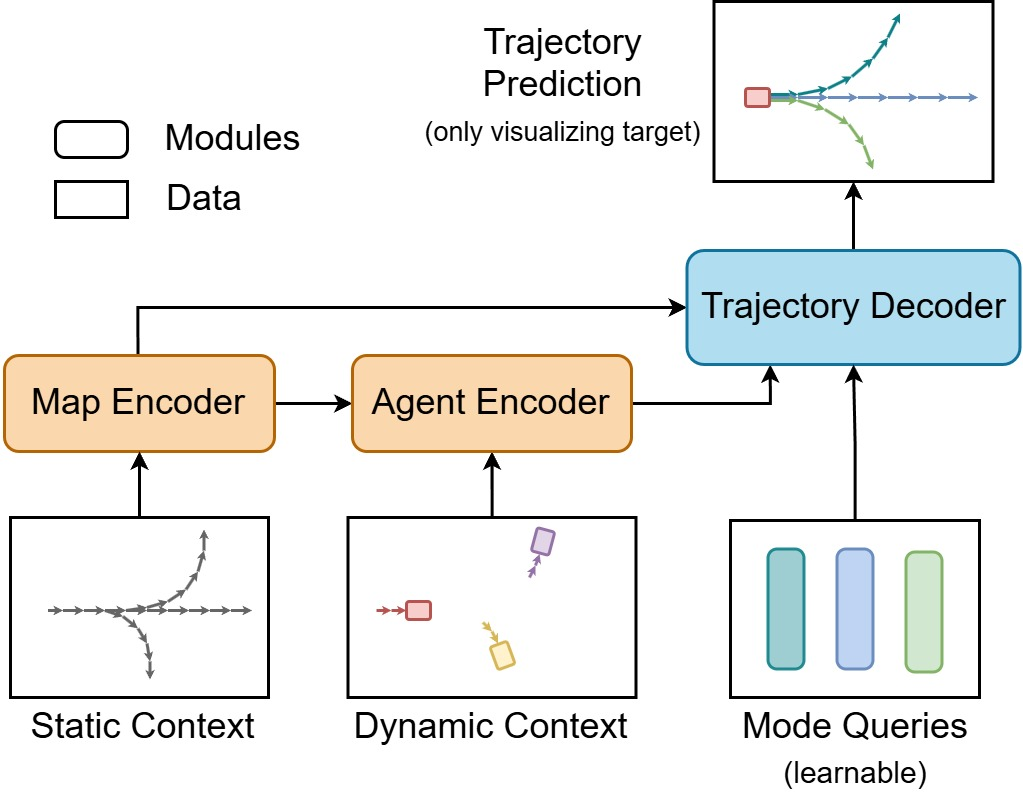
\includegraphics[width=0.9\linewidth]{images/lane_based_prediction_overall_architecture.jpg}
    \caption{An Illustration of LMFormer architecture. We employ a transformer-based encoder-decoder architecture to generate multiple scene-consistent trajectories for all the dynamic agents. Notably the static context only consists of lane segments.}
    \label{fig:overall_net}
\end{figure}

\subsection{Input-Output Formulation}\label{subsection:IO_formulation}
The input to LMFormer consists of the positions of surrounding lanes and dynamic agents in the scene. As described in section \ref{subsection:scene_rep}, we opt for a query-centric representation \cite{zhou2023query} of each scene element. This representation eliminates the need for redundant agent-centric encodings at each time step, thereby reducing the computational overhead associated with repeated coordinate transformations as well as encoding generation. Below, we detail how we compute the query-centric coordinates and features for both static and dynamic contexts. In addition, we also illustrate the formulation of the output trajectory in vector format.

\noindent\textbf{Static Context:} As described in section \ref{subsection:lane_graph}, the static context consists of lane polylines from which lane segments are generated. Every lane segment is characterized by its start and end positions in global coordinates. The query-centric coordinate frame for a lane segment is set as follows: we designate the segment’s start position as its origin and align the segment's vector direction with its x-axis. As a result, the only feature preserved in this query-centric coordinate frame is the segment's length, which we use as its sole feature in the query-centric embedding generation.

\begin{figure}
    \centering
    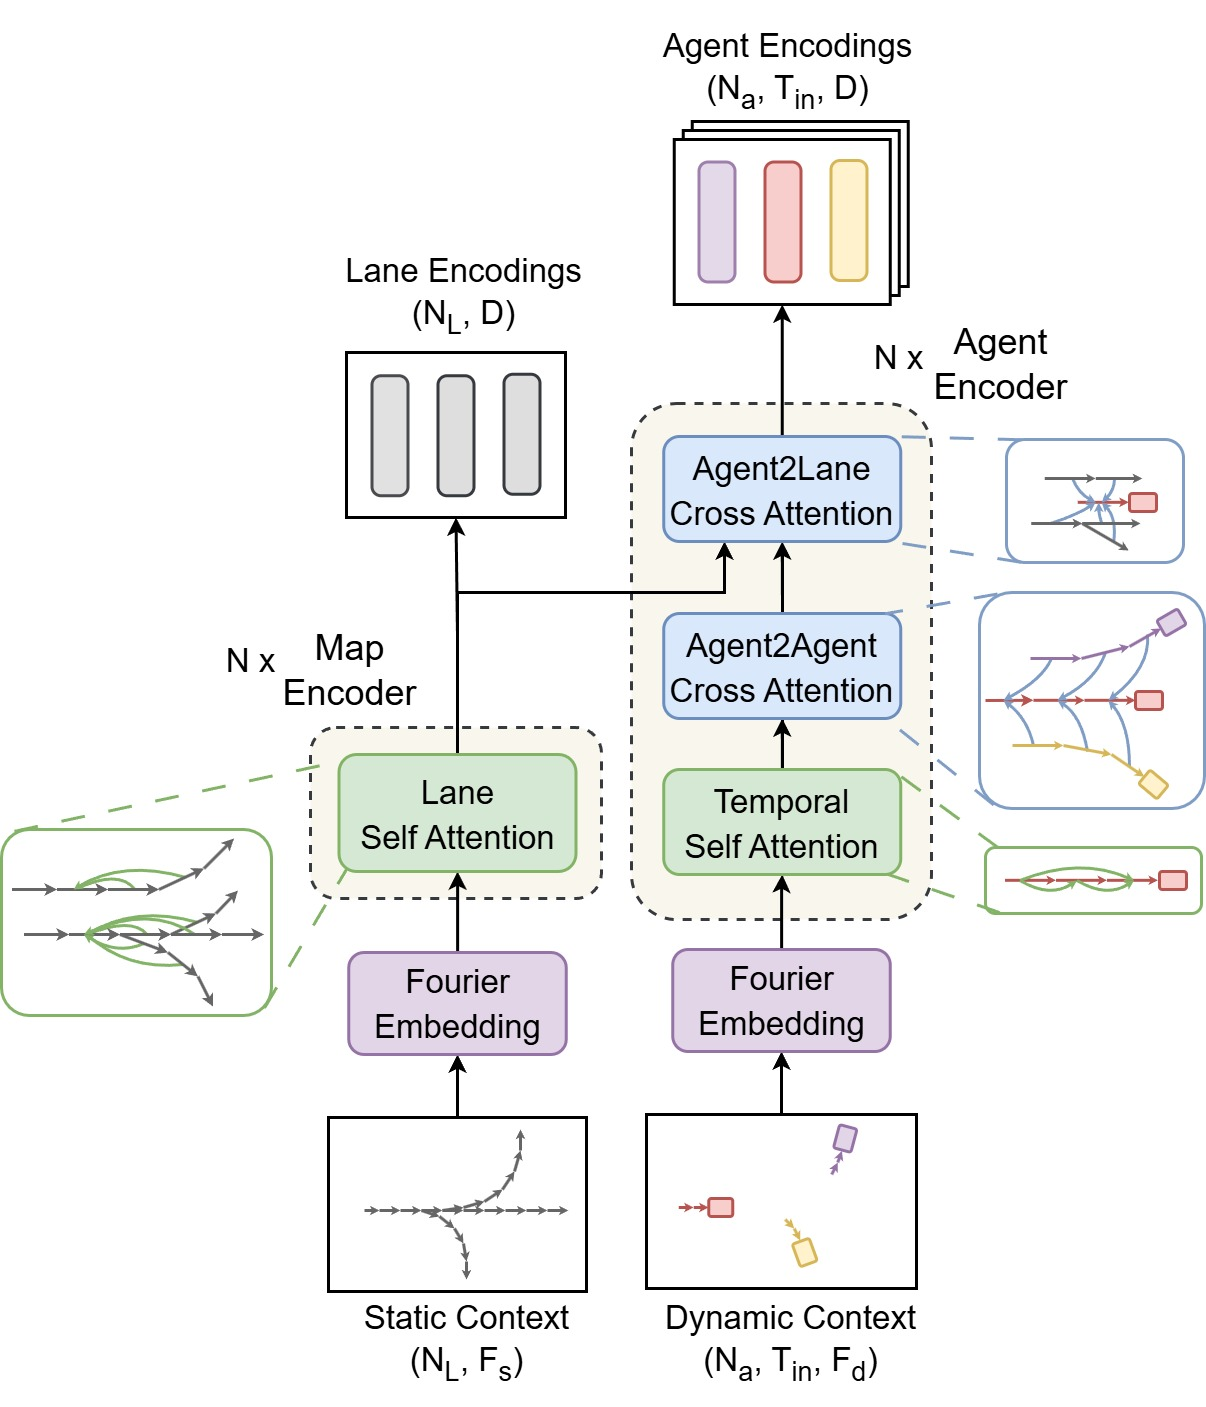
\includegraphics[width=1\linewidth]{images/lane_based_prediction_encoder_paper.jpg}
    \caption{The encoder receives Static and Dynamic context as input and it outputs Lanes and Agents Encodings. The encoder is divided into two parts: Map Encoder and Agent Encoder. The Map Encoder models the long-range interaction among the lane segments. The Agent Encoder models the interaction of all the surrounding static and dynamic elements into each agent's latent embedding. The attention mechanisms are illustrated by green (self-attention) and blue (cross-attention) arrows, where the arrowheads point toward the queries and the tails point away from keys/values. The encoders repeat the interaction modeling N times, to learn complex interactions, where the weights across each layer are not shared.}
    \label{fig:encoder}
\end{figure}

\noindent\textbf{Dynamic Context:} For the dynamic context, agent trajectories are provided as $\mathcal{T}_{in}^a = [P_1^a, P_2^a, ..., P_T^a]$ with global positions $P_t^a$. Motion vectors $M_t^a = [P_t^a, P_{t+1}^a]$ are derived at each time step from these trajectories, encapsulating the agent’s start and end positions within that interval. The query-centric coordinate frame for a motion vector is determined as follows: we set the motion vector’s start position as its origin and align the agent’s instantaneous direction of travel with its x-axis. Notably, the motion vector’s direction may differ from the instantaneous direction of travel, introducing an angular deviation from the x-axis. Consequently, in the query-centric representation, we encode the motion vector’s length and its orientation relative to the x-axis as its features. 

\noindent\textbf{Output Representation:} The output can be represented as  $\mathcal{T}_{out}^{a,m} = [(V_1^{a,m}, S_1^{a,m}), (V_2^{a,m}, S_2^{a,m}), ..., (V_{T'}^{a,m}, S_{T'}^{a,m})]$, where $T'$ is the temporal length of the future trajectories, and $V_t^{a,m} = [P_{t-1}^{a,m}, P_t^{a,m}]$ is the motion vector corresponding to agent $a$, mode $m$, and time step $t$, with an associated variance of $S_t^{a,m}$. The query-centric coordinate frame for these motion vectors is defined as the last observed position and the current direction of travel of the corresponding agent. The predicted future trajectories are reconstructed from these motion vectors in the global coordinate frame, preserving mean positions and associated variances at each time step. Additionally, we predict the probability distribution over predicted trajectories, quantifying the likelihood of each mode.

\subsection{Network Architecture}\label{subsection:network_architecture}
Our model follows a transformer-based encoder-decoder architecture, where the decoder generates scene-consistent trajectories from the latent scene encodings produced by the encoder, as shown in Figure \ref{fig:overall_net}.

\subsubsection{Encoder}\label{subsubsection:encoder}
The encoder is designed to capture interactions between different scene elements. Our design leverages the fact that while the static context is independent of the dynamic context, the reverse does not hold. Consequently, we first encode the static context independently before incorporating it into the dynamic context encoding process. This necessitates two distinct encoders: a Map Encoder and an Agent Encoder, as illustrated in Figure \ref{fig:encoder}. Given the high-frequency nature of motion vectors, we apply learnable Fourier Embeddings \cite{tancik2020fourier} to all scene elements prior to modeling interactions within the encoder.

The Map Encoder is responsible for capturing long-range interactions between lane segments. To construct this interaction graph, we exploit the fact that the most relevant contextual information for each lane segment is present in the lane segments accessible via traversing in the direction of travel. These interactions are modeled using multi-headed attention \cite{vaswani2017attention}, where each lane segment is represented by its query-centric feature embeddings. To capture the relative positions in the multi-headed attention, the keys/values are concatenated with relative position embeddings \cite{zhou2023query}. The Lane Self-Attention module is applied iteratively $N$ times, refining the lane encodings before passing them to the Agent Encoder and subsequent network components.

The Agent Encoder learns interactions between agents and their surrounding scene elements. It comprises three specialized attention modules:
\begin{itemize}
    \item Temporal Self-Attention: Captures dependencies across different time steps for the same agent.
    \item Agent2Agent Cross-Attention: Models interactions between different agents at a given time step.
    \item Agent2Lane Cross-Attention: Encodes contextual interactions from lane segments (keys/values) to agents (queries).
\end{itemize}
Similar to the Map Encoder, multi-headed attention with relative position embeddings is employed in the Agent Encoder. Each interaction module is applied iteratively $N$ times, producing Agent Encodings that serve as input for the trajectory decoder.

\subsubsection{Decoder}\label{subsubsection:decoder}

\begin{figure}
    \centering
    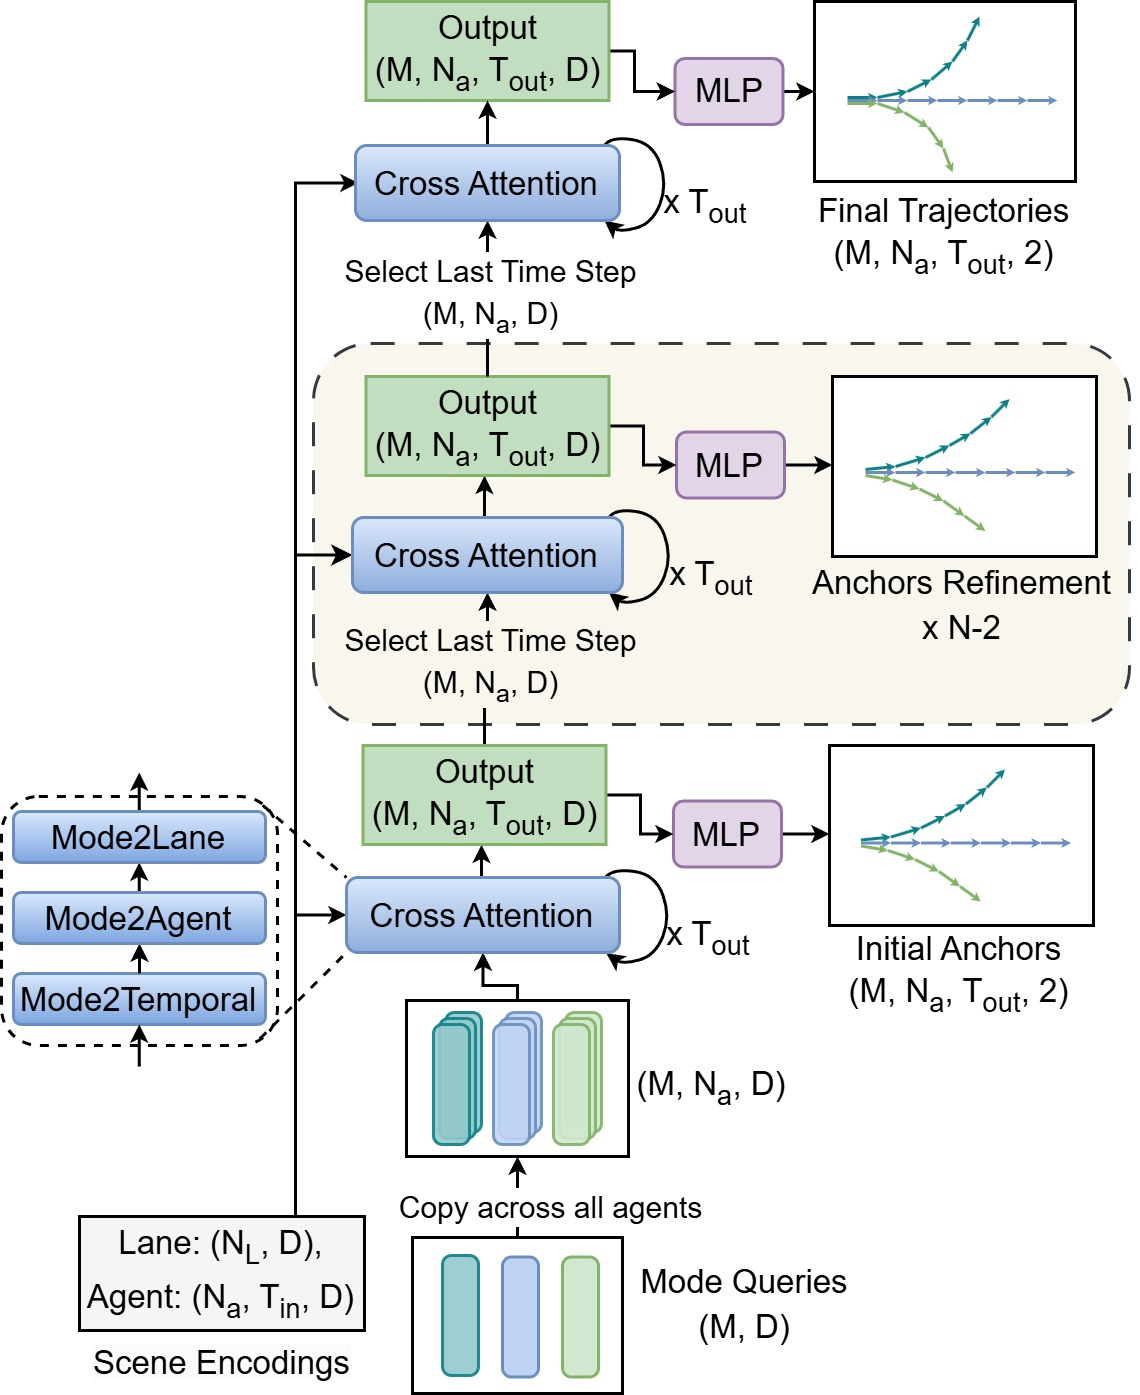
\includegraphics[width=1.\linewidth]{images/lane_based_prediction_decoder_paper.jpg}
    \caption{A depiction of the decoder architecture. The decoder performs cross-attention in between learnable mode queries and Scene Encodings (keys/values). The cross-attention layer is stacked N times and the intermittent output as well as the final output queries are transformed into trajectories with MLP. Thus we obtain N trajectories corresponding to each mode of every agent. During the training, all these N trajectories are trained against the ground truth, while during inference only the final layer output is generated. Importantly, the weights across the stacked cross-attention layers are not shared, while those in the MLP layers are.}
    \label{fig:decoder}
\end{figure}

To facilitate multimodal trajectory prediction, we introduce learnable mode queries, with each query corresponding to a distinct trajectory for every agent in the scene. Figure \ref{fig:decoder} shows the architecture of the decoder.

During initial experiments, we observed that the predicted trajectories exhibited jerky motion and, in some cases, misalignment with lane structures. To mitigate these issues, we drew inspiration from the iterative refinement of bounding boxes in DAB-DETR \cite{liu2022dabdetr}, where bounding boxes are progressively refined through offset computations after each transformer output layer. However, direct adaptation of this approach is impractical for trajectory prediction, as bounding boxes in computer vision are randomly initialized, whereas trajectory prediction requires a reliable set of initial predictions. Thus, instead of applying offset-based refinement at each transformer layer, we compute entire trajectories and compare them against the ground truth to derive additional refinement losses. Another important distinction from DAB-DETR is that LMFormer does not share the weights across each refinement layer, but rather uses the intermittent output from the multiple stacked layers. We show the effectiveness of the additional refinement loss in an ablation study.

Previous research \cite{yadav2025caspformer,zhou2023query} demonstrates that recurrent temporal decoding enhances trajectory prediction quality. Therefore, we incorporate recurrent decoding ($\times T_{out}$) in cross-attention modules. Each recurrent loop updates the query position as well as the query itself, similar to CASPFormer \cite{yadav2025caspformer}. The cross-attention module consists of three key attention mechanisms:
\begin{itemize}
    \item Mode2Temporal Cross Attention: Aggregates temporal information from Agent Encodings (keys/values) to modes (queries).
    \item Mode2Agent Cross Attention: Each mode of an agent attends to the same mode of the other agent in the scene.
    \item Mode2Lane Cross Attention: Enables mode queries to incorporate static context information from Lane Encodings (keys/values).
\end{itemize}

\subsection{Loss Formulation}\label{subsection:loss}
We model the predicted trajectories using a mixture model, which is trained to maximize the likelihood of the ground truth trajectory. The optimization objective is thus formulated as follows:

\begin{equation}
    \mathcal{L}(Y) = \sum_{m=1}^M \pi_m \prod_{t=1}^T P(Y^t | \mu_m^t, b_m^t),
    \label{eq:liklihood_function}
\end{equation}
where $Y$ represents the ground truth trajectory, $\pi_m$ denotes the probability of mode $m$, and $P(\cdot|\cdot)$ follows a Laplace distribution parameterized by the mean $\mu_m$ and scale $b_m$, which defines the positional uncertainty of the predicted trajectories. %In our initial experiments, we also tested Gaussian probability density functions as a candidate for $P(\cdot|\cdot)$, and identified that the network predicts more diverse predictions with the Laplace probability density function.

As shown by Rupprecht et al. \cite{rupprecht2017learning}, directly optimizing the \ac{nll} of mixture models can lead to numerical instability and mode collapse. To mitigate this, the mixture model optimization is decomposed into two objectives via separate regression and classification losses \cite{cui2019multimodal,makansi2019overcoming,zhou2022hivt,yadav2025caspformer}. In our approach, we adopt the \ac{wta} strategy, where the regression loss optimizes only the parameters of the best-matching mode and is defined as:

\begin{align}
    \mathrm{L}_{reg} & = - log \prod_{t=1}^T P(Y^t | \mu_{m*}^t, b_{m*}^t) \nonumber \\
                    & = - \sum_{t=1}^T log \ P(Y^t | \mu_{m*}^t, b_{m*}^t),
\end{align}
where $m^*$ is the mode with the smallest $L_2$ distance to the ground truth trajectory. For the classification loss, we optimize the \ac{nll} of the likelihood function shown in equation \eqref{eq:liklihood_function} as follows:

\begin{equation}
    \mathrm{L}_{cls} = - log \ \mathcal{L}(Y)
\end{equation}

To enhance training stability, we decouple the optimization: the classification loss updates only the mode probabilities $\pi_m$, while the regression loss optimizes the trajectory parameters $\mu_m$ and $b_m$. Finally, the total training loss is defined as the sum of classification and regression losses:

\begin{equation}
    \mathrm{L} = \lambda \ \mathrm{L}_{cls} + \sum_{n=2}^{N}\mathrm{L}_{reg},
\end{equation}
where $N$ denotes the number of stacked layers, and $\lambda$ controls the trade-off between classification and regression losses.